%Laborationsrapport

\documentclass[a4paper,12pt,fleqn]{article}
\usepackage{fixltx2e}
\usepackage[utf8]{inputenc}
\usepackage{graphicx}
\usepackage{sidecap}
\usepackage{fancyhdr}
\usepackage{amssymb,amsmath}
\usepackage[swedish]{babel}
\usepackage[margin=1.5in]{geometry}
\usepackage{abstract}
\usepackage[parfill]{parskip}
\usepackage{tocloft}
\usepackage{adjustbox}
\usepackage{textcomp}
\usepackage[T1]{fontenc}
\usepackage{listings}
\usepackage{xcolor,colortbl}
\usepackage{hyperref}

%----------------------------------------------------------------
%C-kod formatering

\definecolor{listinggray}{gray}{0.9}
\definecolor{lbcolor}{rgb}{0.9,0.9,0.9}
\lstset{
backgroundcolor=\color{lbcolor},
    tabsize=4,    
%   rulecolor=,
    language=[GNU]C++,
        basicstyle=\scriptsize,
        upquote=true,
        aboveskip={1.5\baselineskip},
        columns=fixed,
        showstringspaces=false,
        extendedchars=false,
        breaklines=true,
        prebreak = \raisebox{0ex}[0ex][0ex]{\ensuremath{\hookleftarrow}},
        frame=single,
        numbers=left,
        showtabs=false,
        showspaces=false,
        showstringspaces=false,
        identifierstyle=\ttfamily,
        keywordstyle=\color[rgb]{0,0,1},
        commentstyle=\color[rgb]{0.026,0.112,0.095},
        stringstyle=\color[rgb]{0.627,0.126,0.941},
        numberstyle=\color[rgb]{0.205, 0.142, 0.73},
%        \lstdefinestyle{C++}{language=C++,style=numbers}’.
}
\lstset{
    backgroundcolor=\color{lbcolor},
    tabsize=4,
  language=C++,
  captionpos=b,
  tabsize=3,
  frame=lines,
  numbers=left,
  numberstyle=\tiny,
  numbersep=5pt,
  breaklines=true,
  showstringspaces=false,
  basicstyle=\footnotesize,
%  identifierstyle=\color{magenta},
  keywordstyle=\color[rgb]{0,0,1},
  commentstyle=\color{Darkgreen},
  stringstyle=\color{red}
  }
  %-----------------------------------------------------------------
  %marginaler

  \renewcommand{\abstractnamefont}{\normalfont\normalsize\bfseries}
  \renewcommand{\abstracttextfont}{\normalfont\small}
  \renewcommand{\headrulewidth}{0pt}
  \renewcommand{\cftsecleader}{\cftdotfill{\cftdotsep}} 
  \setlength{\absleftindent}{0pt}
  \setlength{\absrightindent}{0pt}
  \setlength{\headheight}{15pt}

  \addtolength{\oddsidemargin}{-.5in}
  	\addtolength{\evensidemargin}{-.5in}
  	\addtolength{\textwidth}{1in}


  %-----------------------------------------------------------------
  %header and footer

  \pagestyle{fancy}
  \lhead{
  	\begin{picture}(0,0)
  		\put(5,0){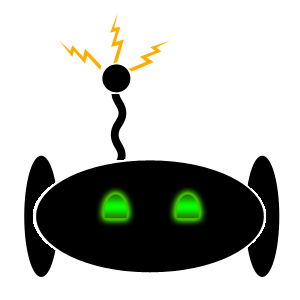
\includegraphics{logotyp.png}}
  	\end{picture}}
	
  \fancyhead[C]{\small{Mapmaster2001}}
  \fancyhead[R]{\small \today}
  \fancyfoot[L]{\small{TSEA56 \\ LIPS Kappa}}
  \fancyfoot[C]{\small{\thepage}}
  \fancyfoot[R]{\small{Projektgrupp 8 \\ mapmaster2001@cyd.liu.se}}

  %-----------------------------------------------------------------

%-------------------------------------------------------------------
%Första sidan

\begin{document}
	\pagestyle{fancy}
\pagenumbering{roman}
	\vspace*{\fill}
		\begingroup
			\begin{center}
				\huge{\textbf{Simultan positionering och kartläggning}}
				\\
				\vspace{10pt}
				\normalsize
				Tobias Grundström och Hans-Filip Elo
				\\
				Kandidatprojekt Y - Grupp 8 - VT2014
				\\
				Version 0.1
				\end{center}
		\endgroup
	\vspace*{\fill}
	
	\begin{center} %Börjar centrering 
		Status
		\\
		\vspace{3pt} %Whitespace 3 pts
	    \begin{tabular}{| p{3cm} | p{3cm} | p{3cm} |} %tabell, 4 horizontella |, 3 cm emellan dem.
	    \hline %översta horizontella linjen.
	    Granskad & - & \today \\ \hline % & -tecken för att "gå till nästa ruta" 
		Godkänd & - & - \\ \hline % avslutas med \\ och \hline.

	    \end{tabular}
	\end{center}
	\vspace{2cm}
	\newpage
%-----------------------------------------------------------------
%Projektidentitet
	
	\vspace*{\fill}
		\begingroup
			\begin{center}
				\LARGE{\textbf{PROJEKTIDENTITET}}
				\\
				\footnotesize
				Grupp 8, 2014/VT, MapMaster2001
				\\
				Linköpings tekniska högskola, ISY
				\\
				\vspace{1cm}
	  \begin{tabular}{| p{3cm} | p{4.3cm} | p{2.4cm} | p{3.8cm} |}
	    \hline
		\textbf{Namn} & \textbf{Ansvar} & \textbf{Telefon} & \textbf{E-post} \\ \hline
	    Jens Edhammer & Dokumentanvsvarig (DOK) & 076-030 67 80 & jened502@student.liu.se \\ \hline
		Erik Ekelund & Designansvarig (DES) & 073-682 43 06 & eriek984@student.liu.se \\ \hline
		David Habrman &  & 976-017 71 15 & davha227@student.liu.se \\ \hline 
		Tobias Grundström & Testansvarig (TES) & 073-830 44 45 & tobgr602@student.liu.se \\ \hline 
		Hans-Filip Elo &   & 073-385 22 32 & hanel742@student.liu.se \\ \hline 
		Niklas Ericson & Projektledare (PL) & 073-052 27 05 & niker917@student.liu.se \\ \hline
	    \end{tabular}
		
		\vspace{1cm}
		\textbf{E-postlista för hela gruppen:} mapmaster2001@cyd.liu.se
		\\[0.5cm]
		
		\textbf{Kund}: Mattias Krysander, Linköpings Universitet, 581 83  LINKÖPING, \\
		013-28 21 98, matkr@isy.liu.se \\
		\textbf{Kontaktperson hos kund}: Mattias Krysander, 013-28 21 98,matkr@isy.liu.se 
		\\
		\textbf{Kursansvarig}: Tomas Svensson, 3B:528,013 28 21 59,tomass@isy.liu.se
		\\[0.5cm]
		\textbf{Handledare}: Peter Johansson, 013-28 1345 peter.a.johansson@liu.se

				\end{center}
		\endgroup
	\vspace*{\fill}
\newpage

%-----------------------------------------------------------------
%Innehållsföreteckning

\addto\captionsswedish{\renewcommand{\contentsname}{Innehållsförteckning}}

\tableofcontents
\thispagestyle{fancy}
\newpage

\pagenumbering{arabic}
%-----------------------------------------------------------------
%Översikt
\section{Inledning}

Simultan positionering och kartläggning (SLAM) är ett problem som kan liknas vid "Hönan och ägget"-problemet. Utan att veta var vi är - hur kartlägger vi då vår omgivining? Åt andra hållet får man ställa sig frågan - hur kartlägger vi vår omgivning utan att veta var vi är? 

Det är inte helt enkelt att lösa dessa frågor, men det finns approximativa på problemet SLAM. Gemensamt för alla lösningar är att de bygger på möjligheten att läsa av sin omgivning i kombination med sannolikhetsteori. Då sensordata aldrig kan antas vara exakt använder sannolikhetsteori för att göra rimlighetsbedömningar i de stickprov av sensordata som sensorerna ger oss. 

Själva problemet är alltså inte entydigt löst rent matematiskt, utan bygger på sannolikhetsteori i kombination med att moderna processorer och minnen kan hantera en stor mängd data. Moderna processorer möjliggör alltså ett stort stickprov vilket leder till en liten osäkerhet. 

\section{Historia}

Principerna för SLAM formulerades för första gången i sin helhet av Smith och Cheeseman (1986). Redan vid formuleringen av problemet menar man på att SLAM är en inexakt vetenskap. SLAM handlar om att skaffa sig en approximativ uppfattning av sin omgivning och position som är tillräckligt bra för att fatta ett beslut kring färdväg och/eller kartläggning. 

Utvecklingen på området har sedan dess accelererats kraftigt tack vare mikrokontrollers förmåga att hantera mer data - då sannolikhetsberäkningarna SLAM innefattar gynnas kraftigt av att arbeta med stora stickprov. 

På senare år har man, precis som inom många andra vetenskapliga områden, sett utvecklingen ta ytterligare ett kliv tack vare internet och öppen källkodsprojekt som Github och OpenSLAM. Att göra en sökning på "SLAM" på Github resulterar i en mängd aktiva projekt på området. Eftersom att källkoden där också finns tillgänglig är detta ett utmärkt exempel för de som vill lära sig om SLAM, undertecknade inkluderade. 

% --------------- Källförteckning ---------------------
\newpage
\section{Källförteckning}
Smith, R.C.; Cheeseman, P. (1986). "On the Representation and Estimation of Spatial Uncertainty". The International Journal of Robotics Research, 5(4), sida 56–68. Hämtad 2014-03-24: \url{http://www.frc.ri.cmu.edu/~hpm/project.archive/reference.file/Smith&Cheeseman.pdf}

% ----------------------------- Appendix -----------------------------------------

\newpage
\appendix
\pagestyle{empty}
\newgeometry{left=2cm,right=2cm,bottom=2cm,top=2cm}
\section{Appendix A}

\end{document}